\documentclass[rnd]{mas_proposal}
% \documentclass[thesis]{mas_proposal}

\usepackage[utf8]{inputenc}
\usepackage{amsmath}
\usepackage{amsfonts}
\usepackage{amssymb}
\usepackage{graphicx}

\title{Testing Deep Neural Networks using Synthetic Dataset Generators}
\author{Rashid Ahamed Meeran Tajdeen}
\supervisors{Prof. Dr. Nico Hochgeschwender (h-brs)\\Deebul Sivarajan Nair (h-brs)}
\date{Dec 2022}

% \thirdpartylogo{path/to/your/image}

\begin{document}

\maketitle

\pagestyle{plain}

\section{Introduction}
    
Though Deep Neural Networks (DNNs) are being used extensively in many fields including safety critical systems such as autonomous driving and medical diagnostics, there are chances for the DNN to exhibit erroneous behaviours. A DNN being developed must undergo a testing process before it gets deployed \cite{DBLP:journals/corr/abs-2112-12591}.

From a software developer point of view, testing a machine learning model would be the white-box testing. But in most cases it is not feasible and are tedious. The most verified process of testing deep neural networks is to test the entire performance without touching the internals of the network. This aspect of testing is more viable and trusted than the other aspects of testing \cite{DBLP:journals/corr/abs-2112-12591}.

Testing is a bit deviating from verification as in testing we run the execution of the product with an aim to find out if it satisfies out need. But during verification the aim is to check if the execution occurs as described in the specification \cite{verification}.
    
\subsection{Why is it essential to test a DNN?}
    
\begin{itemize}
    \item In most DNN image classifiers, the trained models misunderstands one class with the other, or even sometimes show one-sided biases. Hence the properties of the class are violated and misinterpreted.
    \item Some DNNs perform well on simple tasks, but when it comes to the point to expand its use case, the user might begin to face capability issues from the model.
    \item We could never say a DNN model is perfectly trained and can perform well on any situation, because the possibilities real world inputs to this model is infinite.
\end{itemize}
    
\subsection{Challenges in testing DNN?}

\subsubsection{Requires huge input data}
    
Vision based DNNs are completely dependent on the input images. With increase in the size and variability of the input images, its stochastic nature decreases. Hence DNNs require huge input data to train on\cite{ChallengesML}. Getting this huge dataset from realworld even before deploying the product is difficult.

\textbf{Solution:} To overcome the challenge of inadequate data, we propose synthetic image generation which is the creation of artificially generated images that look as realistic as real images. One way to generate these images is by Generation Adversarial Networks(GAN) \cite{9780790} which use a generator-discriminator architecture to train, generate and rate synthetic images multiple times until the generated synthetic image can fool the discriminator enough to be considered a real image. Another way to create synthetic images would be with Variational Autoencoders\cite{9780790}, which create a discrete latent representation and create more variety of images and is easier to train compared to GANs. What if images can be generated by simply typing a short description of the image? In our case this short description would be the requirements from the test engineers. The proposed idea here is to generated synthetic images using blender under certain corner case scenarios and test them on  the trained DNN model. 
    
\subsubsection{Comprehensive white box testing of DNN is costly}
    
Software can be tested using two approaches\cite{verification}. The black-box testing where only the external behaviour of the system is taken into consideration during testing and the white-box testing where the internal working of the system is also taken into consideration.

\textbf{Solution:} The focus here is to test the DNN using the black-box testing approach, in which we test the functionality of the software from the outside. Access to the internals of the DNN is not required in this case and has the advantage to be further scaled to test any type of DNN.

This testing process can be combined with a user defined requirements to make it a Behaviour Driven Development approach. In detail, the testing process is carried out by analysing the performance of the DNN on user defined scenarios.

Testing DNNs must involve the corner-cases to assure reliability\cite{CornerCase}. The user requirements should focus mainly over corner-cases where the data would be abnormal or of type which rarely occurs. These corner-case data can be generated synthetically based on the user requirements.
    
    
\subsection{An example of the testing process}
    
The testing process here can be referred to as a requirement validation process. One sample requirement from the test engineer could be

\quad \textbf{Given} there is a DNN classifier model trained using a particular dataset,

\quad \textbf{When} the model is tested using synthetic images with varying illuminance of 100-200 lux

\quad \textbf{Then} the model must correctly classify the images

During the when step of this requirement, the desired dataset along with its ground truth is generated and classified using the model, and in the then step the results are analysed.

\subsection{Goal of this RnD}
    
The goal of this RnD is to test deep neural networks using requirements validation. The focus is not on investigating the internals of the DNN, instead to test the DNN using formal specifications generated from a set of requirements. To formalise the requirements into specifications, we follow Behaviour Driven Development(BDD) approach. We use synthetic data generator like blender to generate test dataset that are unique to each specifications for testing the performance of the learned DNN models.

\section{Problem Statement}

Over the last decade, Deep Neural Networks(DNNs) have achieved great performance in many domains, such as image processing, medical diagnostics, speech recognition and autonomous driving. 

Similar to traditional software components, DNN models often exhibit erroneous behaviours that may lead to potentially critical errors. Therefore, like traditional software, DNNs needs to be tested effectively to ensure their reliability and safety.

In the software testing context, code coverage criteria are used to guide the generation of test cases and assess the completeness of test suites. But doing that would require a knowledge of the software internals. From the perspective of the user to have the software for a particular application, a well established way to test the DNN is the black-box testing approach in which we analyse the performance of the DNN on certain scenarios. During this process, this work aims to answer the following research questions.

\textbf{Research Questions:}

\begin{itemize}
    \begin{itemize}
        \item[\textbf{RQ1}] What are the state-of-the-art DNN testing approaches?
        \item[\textbf{RQ2}] What are all the parameters that can be varied in blender for dataset generation?
        \item[\textbf{RQ3}] What are the requirements from the test engineer's perspective for testing a vision based DNN?
        \item[\textbf{RQ4}] How to implement BDD for DNN testing based on requirements from test engineers and capabilities of blender?
        \item[\textbf{RQ5}] How the generated synthetic dataset benefits AI testing over real-world dataset?
    \end{itemize}

\end{itemize}


\section{Related Work}
\begin{itemize}
    \item In this paper \cite{DBLP:journals/corr/abs-2112-12591}, the authors investigate black-box input diversity metrics as an alternative to white-box coverage criteria. They first select and adapt three diversity metrics and study, in a controlled manner, their capacity to measure actual diversity in input sets. Then they analyse their statistical association with fault detection using two datasets and three DNN models. They further compare diversity with state-of-the-art white-box coverage criteria. From the experiments, it could be inferred that relying on the diversity of image features embedded in test input sets is a more reliable indicator than coverage criteria to effectively guide the testing of DNNs. One of the selected black-box diversity metrics far outperforms existing coverage criteria in terms of fault-revealing capability and computational time. Results also confirm that state-of-the-art coverage metrics are not adequate to guide the construction of test input sets to detect as many faults as possible with natural inputs.
    
    \item In this paper \cite{DBLP:journals/corr/abs-1803-04792} , inspired by the MC/DC coverage criterion, the authors propose a family of four novel test criteria that are tailored to structural features of DNNs and their semantics. They validate the criteria by demonstrating that the generated test inputs guided via the proposed coverage criteria are able to capture undesired behaviours in a DNN. Test cases are generated using a symbolic approach and a gradient-based heuristic search. By comparing them with existing methods, they prove that their criteria achieve a balance between their ability to find bugs (proxied using adversarial examples) and the computational cost of test case generation. Experiments are conducted on state-of-the-art DNNs obtained using popular open source datasets, including MNIST, CIFAR-10 and ImageNet.
    
    \item In this paper \cite{10.1145/3180155.3180220}, the authors design, implement, and evaluate DeepTest, a systematic testing tool for automatically detecting erroneous behaviors of DNN-driven vehicles that can potentially lead to fatal crashes. A tool is designed to automatically generated test cases leveraging real-world changes in driving conditions like rain, fog, lighting conditions, etc. DeepTest systematically explore different parts of the DNN logic by generating test inputs that maximize the numbers of activated neurons. DeepTest found thousands of erroneous behaviors under different realistic driving conditions (e.g., blurring, rain, fog, etc.) many of which lead to potentially fatal crashes in three top performing DNNs in the Udacity self-driving car challenge.
    
    \item In this paper \cite{9780790}, the authors summarize some of the available tools for creating a synthetic dataset for object segmentation and provide a detailed example using the Blender 3D creation suite. They discuss in detail about the vital points and considerations for automatic dataset generation for object segmentation.
    
    \item There are many parallels between meta-modelling—in the sense of model-driven engineering—and meta-learning. Both rely on abstractions, the meta data, to model a predefined class of problems and to define the variabilities of the models conforming to this definition. Both are used to define the output and input relationships and then fitting the right models to represent that behaviour. In this paper \cite{8906948} , the authors envision how a meta-model for meta-learning can look like. THey discuss possible variabilities, for what types of learning it could be appropriate for, how concrete learning models can be generated from it, and how models can be finally selected. They also discuss a possible integration into existing modelling tools.
    
    \item This survey paper \cite{HUANG2020100270} conducts a review of the current research effort into making DNNs safe and trustworthy, by focusing on four aspects: verification, testing, adversarial attack and defence, and interpretability. In total, they survey 202 papers, most of which were published recently after 2017.
    
    \item In this paper \cite{9283925}, the authors propose a technique that re-purposes software testing methods, specifically mutation-based fuzzing, to augment the training data of DNNs, with the objective of enhancing their robustness. This technique casts the DNN data augmentation problem as an optimization problem. It uses genetic search to generate the most suitable variant of an input data to use for training the DNN, while simultaneously identifying opportunities to accelerate training by skipping augmentation in many instances. They instantiate this technique in two tools, Sensei and Sensei-SA, and evaluate them on 15 DNN models spanning 5 popular image data-sets. The evaluation shows that Sensei can improve the robust accuracy of the DNN, compared to the state of the art, on each of the 15 models, by upto 11.9\% and 5.5\% on average. Further, Sensei-SA reduces the average DNN training time by 25\%, while still improving robust accuracy.
    
\end{itemize}

\section{Project Plan}

\subsection{Work Packages}
The bare minimum will include the following packages:
\begin{enumerate}
    \item[WP1] Literature review on testing of Deep Neural Networks
    \begin{itemize}
        \item[T1.1] Understanding testing of Deep Neural Networks and the concept of synthetic dataset generation.
        \item[T1.2] Literature search on the testing methods introduced in the past.
        \item[T1.3] Identify and analyse the state-of-the-art methods.
    \end{itemize}
    \item[WP2] Experimental setup
    \begin{itemize}
        \item[T2.1] Choose the best synthetic dataset generation tool and analyse its capabilities.
        \item[T2.2] Decide on the DNN models to be used for the testing.
        \item[T2.3] Gather requirements from a test engineer.
        \item[T2.4] Choose a suitable BDD structure that transfers requirements into dataset along with the ground truth.
    \end{itemize}
    \item[WP3] Mid-term Report
    \begin{itemize}
        \item[T3.1] Submission of the mid-term report.
    \end{itemize}
    \item[WP4] Experimental analysis
    \begin{itemize}
        \item[T4.1] Train the DNN model with the synthetic dataset.
        \item[T4.2] Follow a behaviour driven development method.
        \item[T4.3] The Behaviour Driven Development steps creates dataset based on the requirements from the test engineer.
        \item[T4.4] The DNN model is tested using the created dataset.
        \item[T4.5] Analyse the performance of the model.
    \end{itemize}
    \item[WP5] Final Report
    \begin{itemize}
        \item[T5.1] Draft revision.
        \item[T5.2] Submission of the Final report.
    \end{itemize}
    
\end{enumerate}

\subsection{Milestones}
\begin{enumerate}
    \item[M1] Literature search
    \item[M2] Experimental setup
    \item[M3] Mid-term Report submission
    \item[M4] Experimental Analysis
    \item[M5] Final Report submission
\end{enumerate}

\subsection{Project Schedule}
    
\begin{figure}[h!]
    \centering
    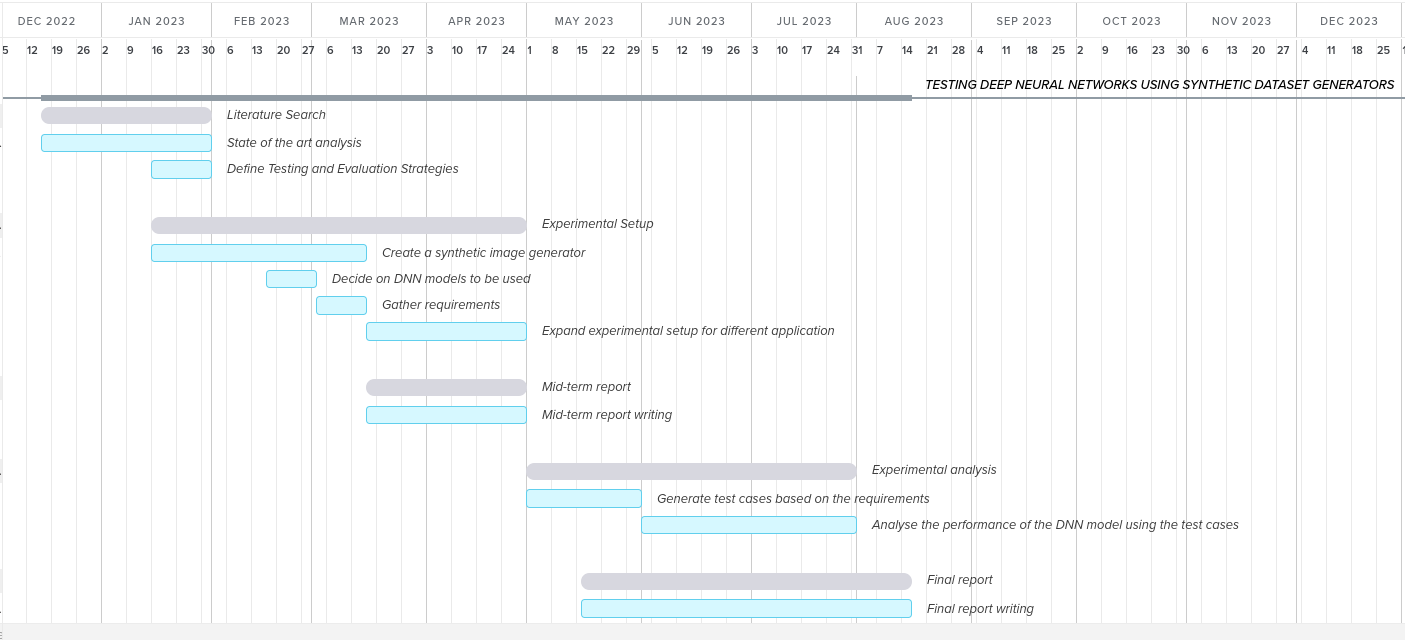
\includegraphics[width=\textwidth]{images/gantt_Dec_15.png}
    \caption{The gantt chart of the RnD project}
    \label{fig:gantt_chart}
\end{figure}

\subsection{Deliverables}
\subsubsection*{Minimum Viable}

\begin{itemize}
    \item State of the art analysis.
    \item A simple and easy to use synthetic dataset generator with variabilies such as illumninance, sharpness, color, contrast, exposure, object poses, camera angles, FOV and perspective.
    \item Training the DNN with the synthetic data generated randomly irrespective of the requirements.
    \item A BDD that could map requirements to dataset generation functions and DNN testing functions.
    \item Testing of the DNN model for a classification or a regression application.
\end{itemize}

\subsubsection*{Expected}
\begin{itemize}
    \item A simple and easy to use synthetic dataset generator with additional variabilities such as material texture and reflection, crowded environment.
    \item Training the DNN with both synthetic and real world data on a ratio 3:1 respectively.
    \item Testing of the DNN model for a classification and a regression application.
\end{itemize}

\subsubsection*{Desired}
\begin{itemize}
    \item An easy to use synthetic dataset generator which could incorporate as much variabilities available in blender.
    \item Training the DNN with relatively more real world data than the synthetic data.
\end{itemize}


\nocite{*}

\bibliographystyle{plainnat} % Use the plainnat bibliography style
\bibliography{bibliography.bib} % Use the bibliography.bib file as the source of references




\end{document}
